% !TeX root=abs_formeln.tex

\subsubsection{Kugeloberfläche}
\begin{equation}\label{eq:mathematik:kreisflaeche}
 A = 4\cdot \pi \cdot r^2
\end{equation}

\subsubsection{Kugelvolumen}
\begin{equation}\label{eq:mathematik:kugelvolumen}
 V = \frac{4}{3}\cdot\pi\cdot r^3
\end{equation}

\subsubsection{pq-Formel}
\begin{equation}\label{eq:mathematik:quadratische:gleichung:pq}
x_{1,2} = - \frac{p}{2} \pm \sqrt{ \left(\frac{p}{2}\right)^2 - q }
\end{equation}
mit $ 0 = x^2 + p \cdot x + q $

\subsubsection{Trigonometrische Beziehungen}
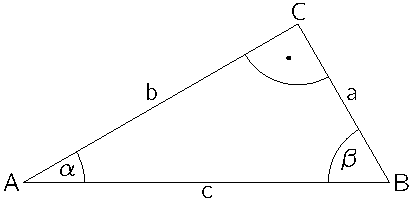
\includegraphics[width=0.6\linewidth]{trigonometrie} \hfill
%\begin{minipage}[b]{.55\linewidth}\raggedright
\begin{align}
\sin\alpha &= \frac{a}{c} = \frac{\text{Gegenkathete}}{\text{Hypotenuse}}\\
\cos\alpha &= \frac{b}{c} = \frac{\text{Ankathete}}{\text{Hypotenuse}}\\
\tan\alpha  &= \frac{a}{b} = \frac{\text{Gegenkathete}}{\text{Ankathete}}
\end{align}
%\end{minipage}
